\subsection{Rendering Views of CAD Models}
\label{sec:dataset-rendering}
Each CAD model of ModelNet is saved in object file format with the extension ".off".
This file contains among others all definitions of faces necessary for modeling the related shape as ASCII text.
Faces refer to an arbitrary number of triangles building a plane.
However, the file starts with the keyword "OFF" and each number of vertices, faces, and edges.
The latter can be ignored because they are not relevant in this representation.
Then, all vertices are listed with each $x$, $y$ and $z$ coordinates, where every vertex is written in a separate line.
This way every vertex has a related index starting at 0.
Afterwards, the faces are listed with one per line.
Every line starts with the number of vertices of this face and then the corresponding vertex indices.
A schematic of this file is shown in \figref{fig:off}.
\begin{figure}
	\centering
	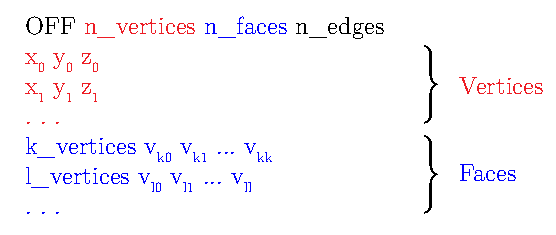
\includegraphics[]{images/off.pdf}
	\caption{CAD Model in Object File Format}
	\label{fig:off}
\end{figure}

The folder structure of ModelNet is as follows.
First, it is divided into training and testing set.
Each set contains identical categories represented as folders.
Within each category folder, the related model files are stored having a unique identifier as their file name.
It is important to mention, that both sets contain different models, hence, if the network is trained on the training set, the models from the test set were never seen before.
Both the sets are recursively searched for models which are then subsequently processed the same way.
How a single model is processed is explained in the following.
All executed operations in Blender are called through a related API call, which allows running those commands for each model in an automated script.

First, the file is imported into Blender, where it is interpreted with respect to its vertices and faces and drawn into a so-called scene.
The origin of the coordinate system of the mesh is set to its center of mass depending on the face areas.
Furthermore, for simplicity, the mesh coordinate system is considered the world coordinate system $\mathcal{W}$.
For adding lighting to the scene a lamp needs to be placed inside.
Blender offers several lamp types, whose effects are shown in \figref{fig:blender-lamps}.
\begin{figure}
	\centering
	\begin{subfigure}{0.19\textwidth}
		\centering
		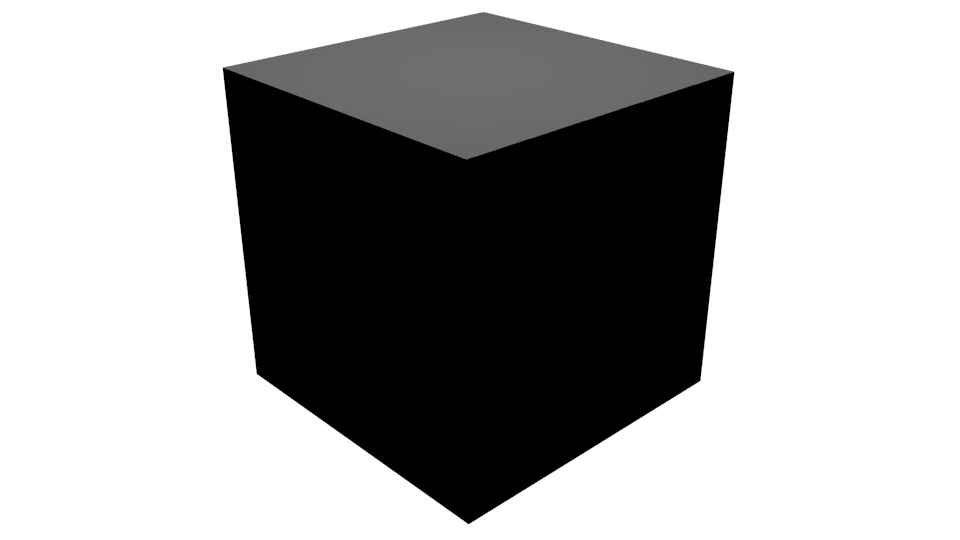
\includegraphics[width=\textwidth]{images/point.png}
		\caption{Point}
	\end{subfigure}
	\begin{subfigure}{0.19\textwidth}
		\centering
		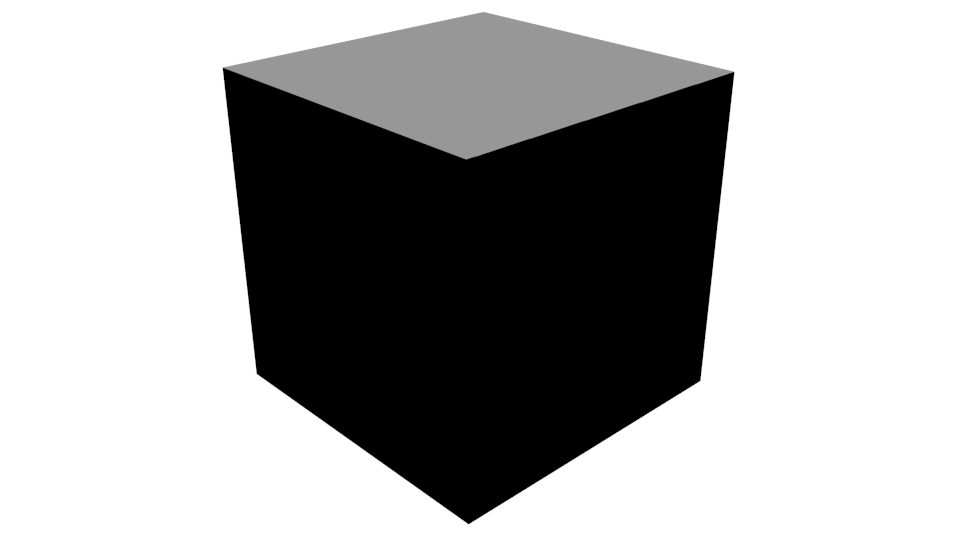
\includegraphics[width=\textwidth]{images/sun.png}
		\caption{Sun}
	\end{subfigure}
	\begin{subfigure}{0.19\textwidth}
		\centering
		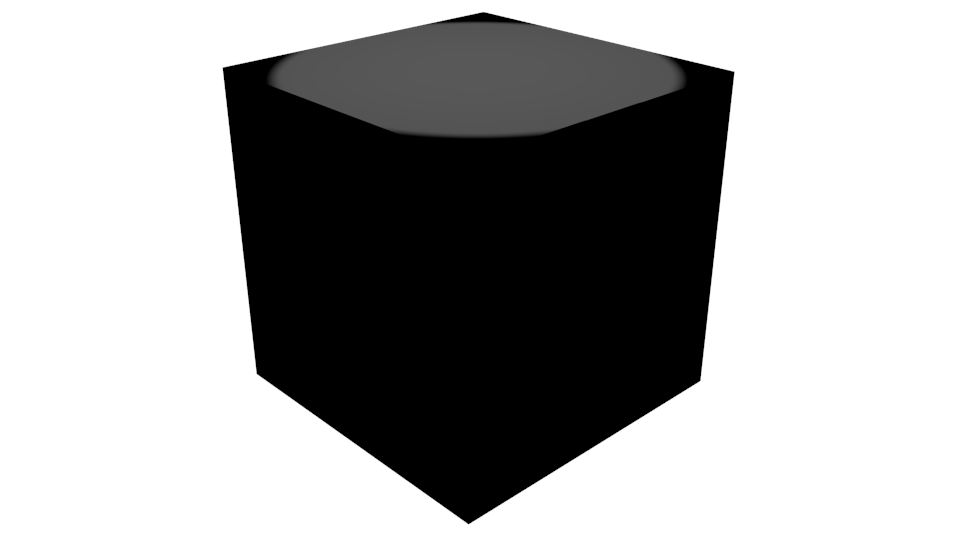
\includegraphics[width=\textwidth]{images/spot.png}
		\caption{Spot}
	\end{subfigure}
	\begin{subfigure}{0.19\textwidth}
		\centering
		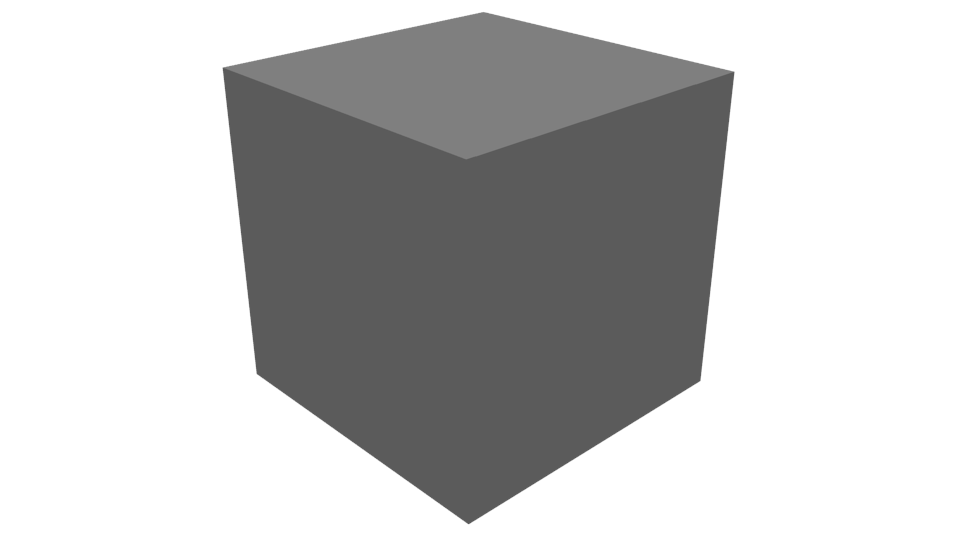
\includegraphics[width=\textwidth]{images/hemi.png}
		\caption{Hemi}
	\end{subfigure}
	\begin{subfigure}{0.19\textwidth}
		\centering
		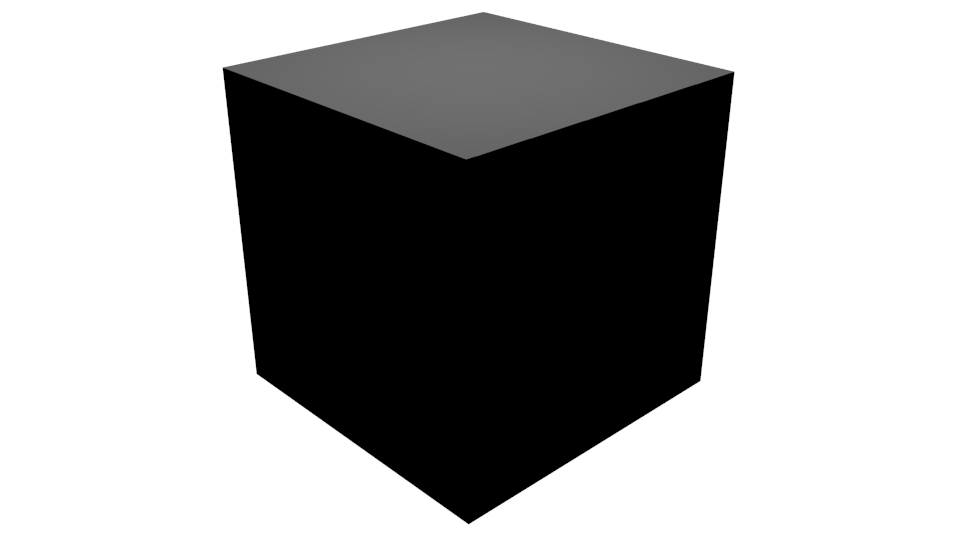
\includegraphics[width=\textwidth]{images/area.png}
		\caption{Area}
	\end{subfigure}
	\caption[Lamp Types Available in Blender]{Lamp types available in Blender. Each light source is placed above the cube pointing directly towards it.}
	\label{fig:blender-lamps}
\end{figure}
The point lamp emits light omnidirectional from its origin.
That means the same amount of light is emitted along the radial direction in all directions.
This is useful for providing local lights like light bulbs.
Another type is the sun lamp.
It is placed very far away and provides light of constant intensity emitted parallel into a single direction.
The spot lamp emits light in a cone-shaped beam into a given direction.
The area lamp is similar to the point lamp, except it emits light from a surface like a TV screen.
This produces shadows with soft borders.
Finally, the hemi lamp emits light radially from a plane.
Similar to the sun lamp, the location is independent, just the direction is important.
One requirement is, that the object should be illuminated on all sides due to the rendering of several views.
Another one is simplicity.
It would get quite complex adding several point lamps for achieving the first requirement.
Hence, the hemi lamp is chosen, assured by \figref{fig:blender-lamps} to provide a well-suited illumination.
Furthermore, although, all models have different heights, a related change of the lamp's location is not necessary due to its properties.
Hence, the lamp is assigned only a rotation of $\vec{r}_l = (0,0,0)^T$, i.e. pointing directly onto the model along the negative $z$-axis.

For rendering views, a camera object $\mathcal{C}$ is necessary and, thus, added to the scene.
Its parameters are left to the default values, except its view distance, which is set very high to work with all models.
Hence, only its location and rotation needs to be set.
Due to the verification from \textit{Su et al.} \cite{Su2018} of the setup from \textit{Su et al.} \cite{Su:2015:MCN:2919332.2919750}, it is adopted.
The camera is elevated 30 degrees from the ground plane, pointing towards its origin.
This results in the first rotation vector
\begin{equation}
	r_{c,0} = \left( \frac{r_{x,deg} \cdot \pi}{180}, 0, 0 \right)^T = \left( \frac{60 \cdot \pi}{180}, 0, 0 \right)^T
\end{equation}
in radians, where $r_{x,deg}$ is the rotation around the $x$-axis in degrees.
Because the camera points along the negative $z$-axis by default, $r_x = 60$ corresponds to the just mentioned setup.
The next step is fitting the camera view to the model just by changing the location of the camera.
Fortunately, Blender supports this with a single API call.
Just like in \cite{Su2018} an image canvas is applied, to support valid convolutions in the future.
This is achieved by moving the camera coordinate system away from the mesh coordinate system along the line of their centers.
However, from the perspective of the camera coordinate system, itself needs to be moved along its $z$-axis, because by definition cameras point towards its negative $z$-axis by default and it is already aligned with the mesh.
Expressing the change of the local camera coordinate system in the mesh coordinate system is done by
\begin{equation}
	\vec{x}_c = \vec{R}_{\mathcal{C} \rightarrow \mathcal{W}} \cdot (\vec{o}_{\mathcal{C}} + \vec{d}) + \vec{t}_{\mathcal{C} \rightarrow \mathcal{W}}
\end{equation}
where the origin $\vec{o}_{\mathcal{C}}$ is moved by $\vec{d}$ first and then rotated and translated according to the difference in both the coordinate systems.
The rotation matrix $\vec{R}_{\mathcal{C} \rightarrow \mathcal{W}}$ and translation vector $\vec{t}_{\mathcal{C} \rightarrow \mathcal{W}}$ are properties directly available in Blender.
The local translation is set to
\begin{equation}
	\vec{d} = \left( 0, 0, \frac{\vec{c}_{\mathcal{W}, z}}{10} \right)^T
\end{equation}
where the $z$ element is a fraction of the original $z$ position $\vec{c}_{\mathcal{W}, z}$ of the camera in the world, i.e the distance from the world origin to the camera object.
The advantage of a fraction is, that the padding is independent of the model's size.
Finally, this camera view is rendered with the following properties.
The resolution is defined to be $224 \times 224$ pixel with a resolution percentage of 100\%.
The latter sets a fraction of the chosen resolution.
This is useful for the development process to save resources and time, but for the final rendering, the full resolution is desired.
Furthermore, it needs to be coped with aliasing.
Because every pixel can only have a single color, edges usually have a step pattern.
This is not realistic, hence, it is smoothed out by anti-aliasing techniques.
This works by rendering the related image region in a higher resolution, taking several samples of pixel values and averaging them to get the value of the pixel in the desired resolution.
The best available sample size in Blender is 16, hence, it is chosen.
The background color is left at the default RGB color $\vec{c} = (64, 64, 64)$ for adding some kind of noise to the views.
A black background would yield inputs of 0 and resembles, in general, no real-world views.
Finally, this view is saved as a PNG file with a trailing view index in its file name, while preserving the original folder structure.
For gathering multiple views, the camera needs to be repositioned.
Hence, the following steps are repeated for the desired number of views.
The rotation of the camera is set to
\begin{equation}
	\vec{r}_c = \left(  \frac{60 \cdot \pi}{180}, 0, \frac{k \cdot s \cdot \pi}{180} \right)^T
\end{equation}
where $k$ is the view index, originally starting at 0, and $s$ the moving interval in degrees.
The latter is set to
\begin{equation}
	s = \frac{360}{n_v} = \frac{360}{12} = 30
\end{equation}
where $n_v$ equals the number of views.
For the ability to compare this work to related researches, $n_v = 12$ is defined.
The number of objects per set corresponds to \cite{Su:2015:MCN:2919332.2919750}.
That means, 90 objects per category for the training set and 30 for the testing set.
However, for simplicity and considering further manipulations with material features, only four categories are picked from the ModelNet10 dataset.
Those embrace bathtubs, dressers, sofas, and monitors.